%! Author = weiss
%! Date = 20.01.2025
\Author{\daAuthorThree}

    This program's backend, which offers a reliable and scalable system for handling all addresses, streets, areas and special features, is the essential layer that makes sure the admin panel and the mobile app for the guides run well. \newline
    This backend serves as the center for data processing and communication, which supports the admin and all guides through a unified API. \newline
    It effectively manages all requests from the mobile app, where guides interact with addresses that are in their area. Furthermore, it manages all necessary requests from the admin panel, which enables accurate management and control over anything relevant for the guides, such as addresses, areas, streets and special features an address may have. \newline 

    One big function of the backend is to enable the admins to perform a wide range of CRUD (Create, Read, Update, Delete) operations on all necessary data. Nevertheless, the other function of the backend is to provide guides with their relevant area and all the addresses in this area. These functionalities are crucial for managing the caroler campaign by the admin and to ensure that the guides have access in the mobile app to accurate and up-to-date addresses and areas. \newline

    We use Spring Boot in our backend which ensures seamless data transfer between the user interfaces (admin panel and mobile app) and the database of this project. By having an organized structure with the different layers (configuration, entities, repositories, services and controllers), we ensure that the system remains flexible, scalable and easy to maintain. \newline 

    Now, this chapter will show the backend's architecture and therefore all its components while also describing how each component functions and contributes to the whole system of the backend.

    \subsection{Config of Spring Boot (application.properties)}
    The \texttt{application.properties} file in our Spring Boot application is the main configuration file where all the necessary settings which are related to the application's behavior are defined. This behavior ranges from the database connection to server properties. In our project, this file ensures that the backend is appropriately configured, so it connects to the database, exposes the API on the correct network address and port, and it makes sure that security settings such as CORS policies are configured right.

        \subsubsection{Database Configuration}
        One of the main functions of the \texttt{application.properties} is to set the database connection. In our case, we utilize the PostgreSQL database and the following properties set the necessary connection details:
        
        \begin{minted}{java}
spring.datasource.driver-class-name=org.postgresql.Driver
spring.datasource.url=jdbc:postgresql://localhost:5432/postgres
spring.datasource.username=postgres
spring.datasource.password=postgres
        \end{minted}
        \captionof{listing}{Database Configuration}
        \begin{itemize}
            \item \texttt{spring.datasource.driver-class-name} defines the driver which is required for the PostgreSQL.
            \item \texttt{spring.datasource.url} sets the connection string to the local database.
            \item \texttt{spring.datasource.username} and \texttt{spring.datasource.password} provide the credentials for the database access on the local computer.
        \end{itemize}
        This configuration ensures that the backend can interact with the local database to store and retrieve all the data efficiently.

        \subsubsection{JPA and Hibernate Settings}
        Spring Boot uses Hibernate for the default JPA implementation. We used the following configuration for this:

        \captionof{listing}{JPA/Hibernate Settings}
        \begin{minted}{java}
spring.jpa.show-sql=true
spring.jpa.properties.hibernate.format_sql=true
spring.jpa.hibernate.ddl-auto=none
spring.jpa.properties.hibernate.dialect= org.hibernate.dialect.PostgreSQLDialect
        \end{minted} 
        
        \begin{itemize}
            \item \textit{spring.jpa.show-sql=true} and \textit{spring.jpa.properties.hibernate.format\_sql=true} enable and format the logging of SQL statements that get executed in the backend.
            \item \textit{spring.jpa.hibernate.ddl-auto=none} ensures that Hibernate does not automatically generate or modify the database tables based on the schemes from the entity classes.
            \item \textit{spring.jpa.properties.hibernate.dialect=org.hibernate.dialect.PostgreSQLDialect} just tells Hibernate to use SQL optimizations which are PostgreSQL-specific.
        \end{itemize}
        
        \subsubsection{Server Configuration}
        The backend application needs to be accessible over a network, and the following configuration sets its address and port:
        \begin{minted}{java}
server.address=0.0.0.0
server.port=46380
server.servlet.context-path=/addresses            
        \end{minted} 
        \captionof{listing}{Server Configuration}

        \begin{itemize}
            \item \texttt{server.address=0.0.0.0} and \texttt{server.port=46380} Set the address and the port of the server.
            \item \texttt{server.servlet.context-path=/addresses} ensures that all API endpoints have the \texttt{/address} prefix.
        \end{itemize}

        \subsubsection{CORS Configuration}
        To allow secure communication between the frontend interfaces (Admin Panel and mobile app), we needed to configure Cross-Origin Resource Sharing (CORS)
        \begin{minted}{java}
spring.web.cors.allowed-origins=https://projektlr.htl-kaindorf.at
spring.web.cors.allowed-methods=GET,POST,PUT,DELETE                      
        \end{minted} 
        \captionof{listing}{CORS Configuration}

        This configuration solved an error we got during the development process.

        \pagebreak
        
    \subsection{Entity Classes (Structure/Purpose)}
    Entity classes use JPA annotations to transfer Java objects to the database as tables. These entity classes are necessary for database interaction to ensure structured data storage and retrieval. \newline
    Each entity, such as addresses, areas, streets and special features of addresses, corresponds to a different concept in the system. However, together they build a relation model that is well-structured and easy to manage. \newline

    \textbf{Annotations:} \newline
    There are several annotations we used in our project to make the entities easier to understand. For example, the area entity looks like this:  
    \begin{minted}{java}
@Data
@Entity
@Table(name = "gebiet")
public class Area {
    @Id
    @GeneratedValue(strategy = GenerationType.IDENTITY)
    @Column(name = "gebietid")
    private Long areaId;
        
    @Column(name = "bezeichnung")
    private String desc;
}                  
    \end{minted} 
    \captionof{listing}{Area Entity}

    In this class, the \texttt{@Data} annotation is used to generate necessary methods like \texttt{Getters} and \texttt{Setters}. \texttt{@Entity} ensures that JPA actually recognizes the class as an entity and \texttt{@Table} is used to give the table of this class a custom name. Furthermore, \texttt{@Id} sets an identifier for the entity. In this case the ID is getting generated automatically with the \texttt{@GeneratedValue} annotation.
    
    \pagebreak
    
    \textbf{Unique identifier:} \newline
    The most important aspect of the backend is handling all the addresses. Every address has a unique identifier, which is defined by a \texttt{house number} and a \texttt{street}. Therefore, we cannot use a single primary key as an identifier for each address. \newline
    The \texttt{AddressId} class is used to manage this composite key. which ensures that each address has its own unique identifier without requiring the generation of an artificial identifier.
    \begin{minted}{java}
@Data
public class AddressId implements Serializable { 
    private String houseNumber;
    private Long streetId;
}                         
    \end{minted} 
    \captionof{listing}{AddressId}

    It is shown in the code snippet from the AddressId class that it uses the mentioned variables as a combination of identifiers, which then results in us not needing to make an artificial identifier like a number that goes up every time the admin adds a new address. \newline

    These composite keys are the best practice if it is not possible to use only one variable as the primary key. This is how the \texttt{AddressId} class is added to the address entity: 
    \begin{minted}{java}
@IdClass(AddressId.class)
public class Address {
    @Id
    @Column(name = "Hausnummer")
    private String houseNumber;

    @Id
    @Column(name = "Strasseid")
    private Long streetId;
}                         
    \end{minted} 
    \captionof{listing}{IDs in Address-Entity}

    The annotation \texttt{@IdClass} has to be used to define what class is used to define the variables of the primary key. Afterwards, the corresponding variables, which are in our case \texttt{houseNumber} and \texttt{streetId}, have to be defined as variables in the entity class. Also, the annotation \texttt{@Id} has to be used over the variables in the entity class to set them as actual IDs. \newline 
    \textbf{Variables in Entities:} \newline \newline
    There are several types of variable types in an entity class. First, the "normal" variable, which has no connection to other entities or is in the ID in any way. These get used for data that is not related to any other entities. This is an example from the address entity of such a variable:
    \begin{minted}{java}
@Column(name = "latitude")
private double latitude;
    
@Column(name = "longitude")
private double longitude;
    
@Column(name = "schonbesucht")
private Boolean alreadyVisited;                     
    \end{minted} 
    \captionof{listing}{"Normal" Variable}

    In this case, these variables save the location data of each address and whether the address had already been visited. It uses the \texttt{@Column} annotation, which is needed because sometimes the name of the column in the database table and the name of the variable in the code may not match for better handling in the code. Otherwise, the variables are just defined with their respective data types. \newline
    The other type of variables are related variables that have a connection to another entity in some way.
    \captionof{listing}{ManyToOne Variable}
    \begin{minted}{java}
@ManyToOne
@JoinColumn(name = "gebietid")
private Area area;
    
@ManyToOne
@JoinColumn(name = "besonderheitid")
private SpecialFeature specialFeature;                    
    \end{minted} 

    This code snippet defines two variables in our address entity that use the \texttt{@ManyToOne} annotation. This is crucial because each address belongs to an area and can have a special feature. We use the IDs from the other entities to make sure that the relationship of the two entities are always right. In this case, because it is a ManyToOne relationship, we did not need to define the address entity in the other classes. \newline

    Sometimes the variables have more complex relationships than just with a simple identifier that gets compared. We had such a case in our project, and it came out like this: 
    \begin{minted}{java}
@ManyToOne(cascade = CascadeType.PERSIST)
@JoinColumns({
@JoinColumn(name = "Strasseid", referencedColumnName = "Strasseid", insertable = false, updatable = false),
@JoinColumn(name = "Postleitzahl", referencedColumnName = "Postleitzahl", insertable = false, updatable = false)
})
private Street street;                   
    \end{minted} 
    \captionof{listing}{Complex ManyToOne Variable}
    This code snippet defines a variable which is related to the street entity. The street entity also has a composite key as its ID so we had to use the \texttt{@JoinColumns} annotation to have a reference to the composite key of the street entity. 

    \subsection{JPA-Repositories (DB Access and CRUD Operations)}
    JPA repositories are a crucial part of the backend to simplify database access by providing methods for many different CRUD (Create, Read, Update, Delete) operations. We utilize repository interfaces that extend \texttt{JpaRepository} instead of manually implementing all these methods that is given to us by the \texttt{JpaRepository}. For example, our \texttt{AddressRepo} interface gets defined like this:  \newline
    \begin{minted}{java}
public interface AddressRepo extends JpaRepository<Address, Integer>{}          
    \end{minted} 
    \captionof{listing}{AddressRepo Interface}
    \pagebreak
    The interface extends \texttt{JpaRepository} with the Address being the entity that gets influenced by the CRUD (Create, Read, Update, Delete) operations and \texttt{Integer} being an id. \newline

    A JPA repository is an interface rather than a normal Java class. We extend an interface with the \texttt{JpaRepository}. By that, we inherit many built-in database methods that make data management significantly easier. Almost any entity class has its own repository interface, which allows us to retrieve, check and manipulate database entries with simple methods calls instead of writing the methods ourselves. \newline

    Such a repository can also set custom methods based on variable names. For example, this code snippet finds a street based on its name and postal code:
    \begin{minted}{java}
Street findStreetByNameAndPostalCode(String name, String postalCode);          
    \end{minted} 
    \captionof{listing}{Find Street By Name And Postal Code}
    As JPA automatically recognizes the method names, these queries do not require any explicit SQL statements.

    \blankLine

    \textbf{Custom Queries with @Query} \newline
    Although JPA simplifies database interactions in many ways, there are some specific cases where automatic query generation does not work. In our project, we encountered an issue where Hibernate had problems correctly inserting a new address into the table. To solve this problem, we had to create this custom SQL query in the repository:
    \begin{minted}{java}
@Modifying
@Transactional
@Query(value = "INSERT INTO adresse (hausnummer, strasseid, postleitzahl, latitude, longitude, besonderheitid, gebietid, schonbesucht, kommentar)" +
       "VALUES (:houseNumber, :streetId, :postalCode, :latitude, :longitude, :specialFeatureId, :areaId, :alreadyVisited, :comment);",
       nativeQuery = true)
int insertAddress(@Param("houseNumber") String houseNumber,
                  @Param("streetId") Long streetId,
                  @Param("postalCode") String postalCode,
                  ...);          
    \end{minted} 
    \captionof{listing}{Insert Address with Custom Query}

    This method inserts a new address with all its variables into the database, but it requires additional annotations.
    \begin{itemize}
        \item \texttt{@Query:} Specifies the custom SQL query that has to be executed.
        \item \texttt{@Modifying:} Indicates that this particular query modifies the database, which would not be needed if it were only a \texttt{SELECT} statement.
        \item \texttt{@Transactional:} Ensures that the query runs in a transaction, which prevents issues like incomplete data insertion.
        \item \texttt{@Param:} Is needed so the parameters are placeholders in the SQL statement.
    \end{itemize}

    \subsection{Service Classes}
    Service classes contain the logic for the database interaction and serve as a bridge between the controllers and repositories. Before passing data to controllers or repositories, they handle data retrieval and manipulation of the data.

    \subsubsection{@Service Annotation}
    The \texttt{@Service} annotation is used to define a class as an actual service component. It originates from the \texttt{@Component} annotation, which makes it eligible for Spring's component scanning and dependency injection. \newline
    Every service class interacts with at least one repository, which gets injected through a constructor-based dependency injection using the \texttt{@Autowired} annotation. This injection looks like this in the service class: 
    \begin{minted}{java}
@Service
public class AddressService {        
    private final AddressRepo addressRepo;
    private final AreaRepo areaRepo;
    ...

    @Autowired
    public AddressService(AddressRepo addressRepo, AreaRepo areaRepo, StreetRepo streetRepo, SpecialFeatureRepo specialFeatureRepo) {
        this.addressRepo = addressRepo;
        this.areaRepo = areaRepo;
        ...
    }
}
    \end{minted}
    \captionof{listing}{Repository Injection and @Service}
    Here \texttt{AddressService} depends on many repositories, and Spring automatically injects the required interface. 

    \subsubsection{Repository Usage in Service Methods}
    Now that the service class has all the necessary repositories, it has to use the methods too. Some common operations look like this: \newline
    This method returns all addresses in the database: 
    \begin{minted}{java}
public List<Address> getAllAddresses() {
    return addressRepo.findAll();
}
    \end{minted}
    \captionof{listing}{Fetching all Addresses}

    \blankLine

    In this case, it toggles if the address has already been visited or not:
    \begin{minted}{java}
public Address toggleAlreadyVisited(String houseNumber, Long streetId) {
    Address address = addressRepo.findAddressByHouseNumberAndStreetId(houseNumber, streetId);
    
    address.setAlreadyVisited(address.getAlreadyVisited() == null || !address.getAlreadyVisited());
    
    log.info(address.toString());
    
    return addressRepo.save(address);
}
    \end{minted}
    \captionof{listing}{Toggle Already Visited}

    And that inserts a new address with the custom query from the \texttt{AddressRepo}: 
    \begin{minted}{java}
@Transactional
public void createNewAddress(
    String houseNumber,
    double lat,
    double lng,
    ...
) {
    int insert = addressRepo.insertAddress(
                    address.getHouseNumber(),
                    address.getStreetId(),
                    address.getStreet().getPostalCode(),
                    ...
    );
}    
    \end{minted}
    \captionof{listing}{Insert new Address}

    These methods from the repositories are used in almost every function of the service class. From retrieving data to creating a new address, there are many methods that are built-in or can be easily created in the repository classes that get used by the service classes.

    \subsubsection{Computing Border Addresses Using Convex Hull}
    An important function of the backend is to calculate the border addresses that are around a given area. This function is implemented in the \texttt{AddressService} class. In this case, the \texttt{getBorderAddresses} method calculates the convex hull from this given area. The main method uses many helper methods and an extra class, so the calculation does not use that much resources. 
    
    \pagebreak
    
    \textbf{Point Class} \newline
    To calculate the convex hull, we use the longitude and latitude of the addresses in an area. Processing every address with all its fields would cost much more resources than only using the longitude and latitude of every address. That is the purpose of the \texttt{Point} class. It looks like this: 
    \begin{minted}{java}
@AllArgsConstructor
@Data
public class Point {
    private double longitude;
    private double latitude;
}
    \end{minted}
    \captionof{listing}{Point Class}
    This class only saves the longitude and latitude of an address to save a bit more resources. \newline

    \textbf{Helper Methods} \newline
    There are some methods we created that get used in the main method to get the border addresses to make it easier to understand what each method does. 
    \textbf{PolarAngle}
    The \texttt{polarAngle} method is used to calculate the polar angle between two points so that it can be used to find out which points are the nearest and can be compared to each other next. This method is implemented like this: 
    \begin{minted}{java}
public double polarAngle(Point origin, Point point) {
    return Math.atan2(point.getLongitude() - origin.getLongitude(), point.getLatitude() - origin.getLatitude());
}
    \end{minted}
    \captionof{listing}{Polar Angle Method}
    The method gets two points and compares them to each other with the \texttt{Math.atan2} method, which is provided by the \texttt{Math} package. \newline

    \textbf{IsCounterClockwise} \newline
    The \texttt{isCounterClockwise} method is used to check if three points are counterclockwise. This is important to make sure the convex hull is actually convex and not concave. The method to calculate this looks like this: 
    \begin{minted}{java}
public boolean isCounterClockwise(Point p1, Point p2, Point p3) {
    return (p2.getLatitude() - p1.getLatitude()) * (p3.getLongitude() - p1.getLongitude()) - (p2.getLongitude() - p1.getLongitude()) * (p3.getLatitude() - p1.getLatitude()) > 0;
}
    \end{minted}
    \captionof{listing}{is Counter Clockwise Method}

    \textbf{Convex Hull}
    
    The \texttt{convexHull} method uses the helper methods and other logic to return the convex hull. The method gets a list of points. \newline
    
    The \texttt{convexHull} method starts with a clause that may directly stop the calculation. To build a convex hull, there have to be at least four points, so if there are less than four points, the method returns an empty list.
    \captionof{listing}{if Clause for Point Size}
    \begin{minted}{java}
if (points.size() < 3) {
    return Collections.emptyList();
}
    \end{minted}
 
    If there are enough points, the actual \texttt{convexHull} can start. First, it finds the lowest point based on the latitude or the leftmost point if the latitudes of the two lowest points are the same. It goes through all the points given to the method and compares the latitude.
    \begin{minted}{java}
Point lowest = points.stream()
    .min(Comparator.comparing(
            Point::getLatitude
        ).thenComparing(Point::getLongitude))
    .orElse(null);
    \end{minted}
    \captionof{listing}{Lowest Point Calculation}

    Then, using one of the helper methods, the program sorts the points based on their polar angles to each other. This is relatively easy to do by given a comparator provided by Java.

    \begin{minted}{java}
points.sort(Comparator.comparingDouble(p -> polarAngle(lowest, p)));
    \end{minted}
    \captionof{listing}{Sort Points Based on Polar Angle}

    Afterwards, the method creates a stack and adds the first two points of the sorted list to the stack. 
    \begin{minted}{java}
Stack<Point> stack = new Stack<>();
stack.push(points.get(0));
stack.push(points.get(1));
    \end{minted}
    \captionof{listing}{Create Stack}

    After the stack is created, the program goes through a loop that goes through every point in the list. In the loop, it creates a new variable that always gets the last added point of the stack and uses it as a reference point. Then the other helper method is used to look if the next point of the list is in the convex hull. If the next point is in the convex hull, then it gets added to the stack. This stack is then returned as a list for later processing.
    \begin{minted}{java}
for (int i = 2; i < points.size(); i++) {
    Point top = stack.pop();

    while (!stack.isEmpty() && !isCounterClockwise(stack.peek(), top, points.get(i))) {
        log.info("Popping point: " + top);
            top = stack.pop(); // Removes top until the border makes a left turn
        }

    log.info("Pushing point: " + points.get(i));

    stack.push(top);
    stack.push(points.get(i));
}

return new ArrayList<>(stack);
    \end{minted}
    \captionof{listing}{Convex Hull Calculation}

    In the \texttt{getBorderAddresses} method, the \texttt{convexHull} method is used, and the convex hull points are stored in a list. Furthermore, this list gets used to add a tolerance to every point. This is the case because we encountered some issues while creating this convex hull, and we found out by adding a bit of tolerance that this issue was fixed. This is because the locations of the addresses are not precise enough. After adding this tolerance, the list of points that build the convex hull is returned.
    \begin{minted}{java}
List<Point> hull = convexHull(points);

List<Address> borderAddresses = new ArrayList<>();
        
for (Point p : hull) {
    for (Address address : addresses) {
        double latDiff = Math.abs(address.getLatitude() - p.getLatitude());
        double lonDiff = Math.abs(address.getLongitude() - p.getLongitude());
        
        if (latDiff < TOLERANCE && lonDiff < TOLERANCE) {
            borderAddresses.add(address);
            break;
        }
    }
}
        
return borderAddresses;
    \end{minted}
    \captionof{listing}{Lowest Point Calculation}

    \subsection{Rest Controller (API Endpoints and their Functions)}

    REST controllers expose API endpoints that handle HTTP requests and then return the appropriate responses. These controllers allow the frontend interfaces (Admin Panel and mobile app) to interact in any way with the backend to perform operations like retrieving, updating and deleting data. In our project, two main REST controllers are responsible for handling all the tasks: the \texttt{AddressController} and the \texttt{AdminController}.

    \pagebreak

    \subsubsection{AddressController}
    The \texttt{AddressController} class is for handling endpoints for the guides and the mobile app and provides the necesssary functions to retrieve and update certain information. Each method in this controller corresponds to a certain operation the guides can do. These are the endpoints the \texttt{AddressController} exposes to the network: \newline \newline
    \textbf{GET Routes} 
    \begin{enumerate}
        \item \textbf{\texttt{GET /} - Get All Addresses}
        \begin{itemize}
            \item This endpoint gets a list of all addresses stored in the system. 
            \item It is mostly used to display the addresses in the mobile app.
        \end{itemize} 
        \begin{figure} [H]
            \centering
            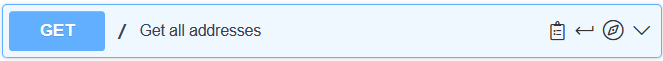
\includegraphics [width=1\textwidth] {images/andreas/praxis/getAllAddresses.png}
            \caption{Get Route for all Addresses}
        \end{figure}

        \item \textbf{\texttt{GET /{area}} - Get All Addresses Of An Area}
        \begin{itemize}
            \item This endpoint allows users to get a list of addresses from a specific area.
            \item The area is provided as a path variable
        \end{itemize}
        \begin{figure} [H]
            \centering
            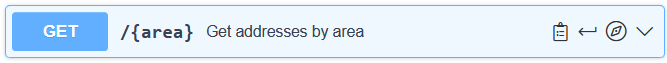
\includegraphics [width=1\textwidth] {images/andreas/praxis/getAddressesByArea.png}
            \caption{Get Route for all Addresses by Area}
        \end{figure}

        \item \textbf{\texttt{GET /{area}/borderAddress} - Get Border Addresses}
        \begin{itemize}
            \item This endpoint gives the frontend the border addresses of the convex hull of an area.
        \end{itemize} 
        \begin{figure} [H]
            \centering
            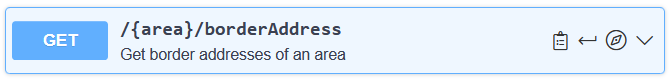
\includegraphics [width=1\textwidth] {images/andreas/praxis/getBorderAddressesOfArea.png}
            \caption{Get Route for Border Addresses by Area}
        \end{figure}
    \end{enumerate}    

    \textbf{PUT Routes}

    \begin{enumerate}    
        \item \textbf{\texttt{PUT /{streetId}/{houseNumber}/toggleVisited} - Toggle Visited Status}
        \begin{itemize}
            \item This endpoint allows toggling the "visited" status of a specific address.
        \end{itemize} 
        \begin{figure} [H]
            \centering
            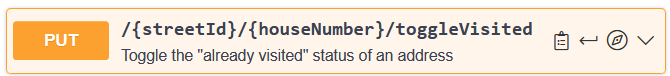
\includegraphics [width=1\textwidth] {images/andreas/praxis/toggleAlreadyVisitedOfAddress.png}
            \caption{Put Route to Toggle Visited}
        \end{figure}

        \item \textbf{\texttt{PUT /{streetName}/{postalCode}/toggleAlreadyVisitedOnStreet}}
        \begin{itemize}
            \item This endpoint updates the "visited" status for all addresses on a particular street, marking them as either visited or not.
        \end{itemize} 
        \begin{figure} [H]
            \centering
            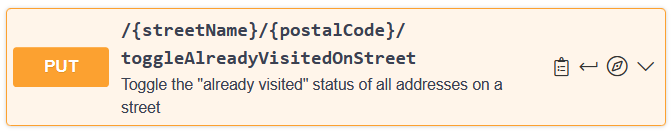
\includegraphics [width=1\textwidth] {images/andreas/praxis/toggleAlreadyVisitedOfAddressesOnStreet.png}
            \caption{Put Route to Toggle Whole Street Visited}
        \end{figure}

        
    \end{enumerate}

    \subsubsection{Admin Controller}
    This controller has all the endpoints relevant to managing the data. These routes are not meant for the guides from the mobile app, they are here for the admin in the Admin Panel. These routes are for the admin to use: \newline \newline
    \textbf{GET Routes}
    \begin{enumerate}
        \item \textbf{\texttt{GET /getAllStreets} - Get All Streets}
        \begin{itemize}
            \item This endpoint retrieves a list of all streets in the system.
        \end{itemize} 
        \begin{figure} [H]
            \centering
            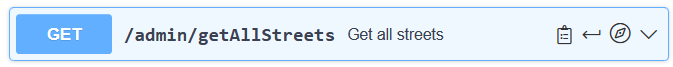
\includegraphics [width=1\textwidth] {images/andreas/praxis/getAllStreets.png}
            \caption{Get Route for all Streets}
        \end{figure}

        \item \textbf{\texttt{GET /getAllAreas} - Get All Areas}
        \begin{itemize}
            \item This endpoint returns a list of all areas in the system.
        \end{itemize} 
        \begin{figure} [H]
            \centering
            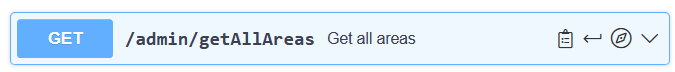
\includegraphics [width=1\textwidth] {images/andreas/praxis/getAllAreas.png}
            \caption{Get Route for all Areas}
        \end{figure}

        \item \textbf{\texttt{GET /getAllSpecialFeatures} - Get All Special Features}
        \begin{itemize}
            \item This endpoint retrieves all special features present in the system.
        \end{itemize} 
        \begin{figure} [H]
            \centering
            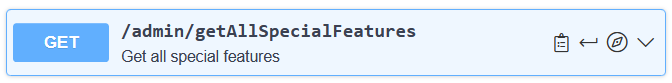
\includegraphics [width=1\textwidth] {images/andreas/praxis/getAllSF.png}
            \caption{Get Route for all Special Features}
        \end{figure}
    \end{enumerate}

    \textbf{PUT Routes}
    \begin{enumerate}
        \item \textbf{\texttt{PUT /updateComment} - Update Address Comment}
        \begin{itemize}
            \item This endpoint allows updating the comment associated with an address.
        \end{itemize} 
        \begin{figure} [H]
            \centering
            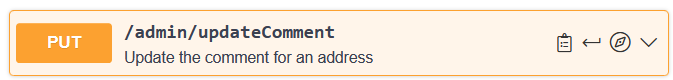
\includegraphics [width=1\textwidth] {images/andreas/praxis/updateComment.png}
            \caption{Put Route to Update Comment on Address}
        \end{figure}

        \item \textbf{\texttt{PUT /updateAddressesByRange} - Update Addresses by Range}
        \begin{itemize}
            \item This endpoint updates the area of addresses based on a range of house numbers within a street
        \end{itemize} 
        \begin{figure} [H]
            \centering
            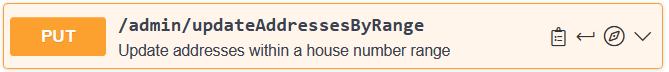
\includegraphics [width=1\textwidth] {images/andreas/praxis/updateAddressesHouseRange.png}
            \caption{Put Route to Update Addresses by Range}
        \end{figure}

        \item \textbf{\texttt{PUT /updateAddressesByParity} - Update Addresses by Parity (Odd/Even)}
        \begin{itemize}
            \item This endpoint updates addresses based on their house number parity (odd or even).
        \end{itemize} 
        \begin{figure} [H]
            \centering
            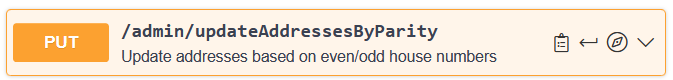
\includegraphics [width=1\textwidth] {images/andreas/praxis/updateAddressesOddEven.png}
            \caption{Put Route to Update Address by Odd/Even}
        \end{figure}

        \item \textbf{\texttt{PUT /updateAddressesByList/{areaDesc}} - Update Addresses by List}
        \begin{itemize}
            \item This endpoint allows bulk updates to a list of addresses, changing the any variable of each address in the provided list.
        \end{itemize} 
        \begin{figure} [H]
            \centering
            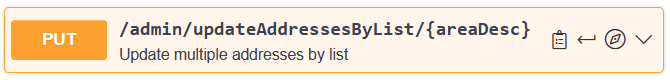
\includegraphics [width=1\textwidth] {images/andreas/praxis/updateAddressByList.png}
            \caption{Put Route to Update all Addresses in a Custom List}
        \end{figure}

        \item \textbf{\texttt{PUT /editArea} - Edit Area Information}
        \begin{itemize}
            \item This endpoint allows modification of an area’s description and associated details.
        \end{itemize} 
        \begin{figure} [H]
            \centering
            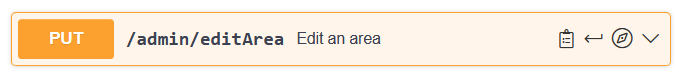
\includegraphics [width=1\textwidth] {images/andreas/praxis/editArea.png}
            \caption{Put Route to Edit an Area}
        \end{figure}

        \item \textbf{\texttt{PUT /setSpecialFeature} - Set Special Feature for Address}
        \begin{itemize}
            \item This endpoint assigns a special feature to an address.
        \end{itemize} 
        \begin{figure} [H]
            \centering
            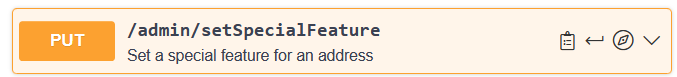
\includegraphics [width=1\textwidth] {images/andreas/praxis/setSFOfAddress.png}
            \caption{Put Route to Set Special Feature on Address}
        \end{figure}

        \item \textbf{\texttt{PUT /editAddress} - Edit an Address}
        \begin{itemize}
            \item This endpoint allows the modification of an existing address, such as updating its house number, street name, or additional details.
        \end{itemize} 
        \begin{figure} [H]
            \centering
            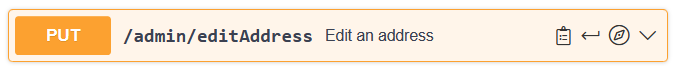
\includegraphics [width=1\textwidth] {images/andreas/praxis/editAddress.png}
            \caption{Put Route to Edit an Address}
        \end{figure}

        \item \textbf{\texttt{PUT /editAddresses} - Edit Multiple Addresses}
        \begin{itemize}
            \item This endpoint allows bulk edits to multiple addresses at once, facilitating large-scale updates.
        \end{itemize} 
        \begin{figure} [H]
            \centering
            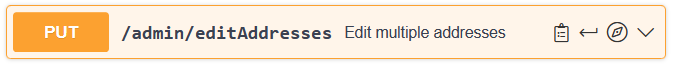
\includegraphics [width=1\textwidth] {images/andreas/praxis/editAddresses.png}
            \caption{Put Route to Edit Multiple Addresses}
        \end{figure}

        \item \textbf{\texttt{PUT /editSpecialFeature} - Edit Special Feature}
        \begin{itemize}
            \item This endpoint allows editing a special feature that is already existing in the database.
        \end{itemize} 
        \begin{figure} [H]
            \centering
            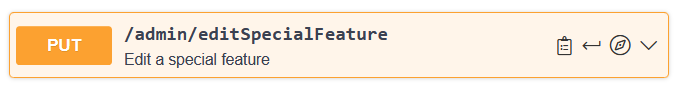
\includegraphics [width=1\textwidth] {images/andreas/praxis/editSF.png}
            \caption{Put Route to Edit Special Feature}
        \end{figure}
    \end{enumerate}

    \pagebreak

    \textbf{POST Routes}
    \begin{enumerate}
        \item \textbf{\texttt{POST /addAddress} - Add a New Address}
        \begin{itemize}
            \item This endpoint allows the creation of a new address record.
            \item All relevant details such as house number, street name, postal code, and coordinates must be provided.
        \end{itemize} 
        \begin{figure} [H]
            \centering
            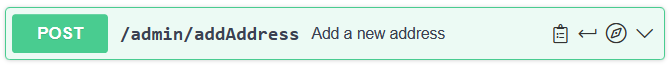
\includegraphics [width=1\textwidth] {images/andreas/praxis/addAddress.png}
            \caption{Post Route to Create an Address}
        \end{figure}

        \item \textbf{\texttt{POST /addStreet} - Add a New Street}
        \begin{itemize}
            \item This endpoint creates a new street record, specifying its name and postal code.
        \end{itemize} 
        \begin{figure} [H]
            \centering
            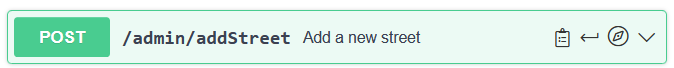
\includegraphics [width=1\textwidth] {images/andreas/praxis/addStreet.png}
            \caption{Post Route to Create a Street}
        \end{figure}

        \item \textbf{\texttt{POST /addArea/{areaDesc}} - Add a New Area}
        \begin{itemize}
            \item This endpoint allows the addition of a new area to the system.
        \end{itemize} 
        \begin{figure} [H]
            \centering
            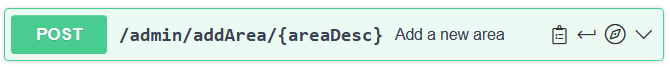
\includegraphics [width=1\textwidth] {images/andreas/praxis/addArea.png}
            \caption{Post Route to Create an Area}
        \end{figure}

        \item \textbf{\texttt{POST /addSpecialFeature} - Add a New Special Feature}
        \begin{itemize}
            \item This endpoint creates a new special feature.
        \end{itemize} 
        \begin{figure} [H]
            \centering
            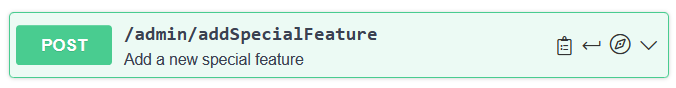
\includegraphics [width=1\textwidth] {images/andreas/praxis/addSF.png}
            \caption{Post Route to Create a Special Feature}
        \end{figure}
    \end{enumerate}

    \textbf{DELETE Routes}
    \begin{enumerate}
        \item \textbf{\texttt{DELETE /deleteStreet} - Delete a Street}
        \begin{itemize}
            \item This endpoint deletes a street from the system.
        \end{itemize} 
        \begin{figure} [H]
            \centering
            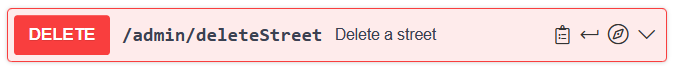
\includegraphics [width=1\textwidth] {images/andreas/praxis/deleteStreet.png}
            \caption{Delete Route to Delete a Street}
        \end{figure}

        \item \textbf{\texttt{DELETE /deleteArea} - Delete an Area}
        \begin{itemize}
            \item This endpoint deletes an area from the system.
            \item All addresses in that area may need to be reassigned or deleted as well.
        \end{itemize} 
        \begin{figure} [H]
            \centering
            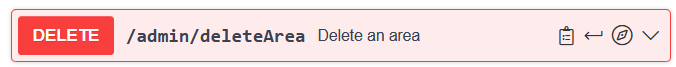
\includegraphics [width=1\textwidth] {images/andreas/praxis/deleteArea.png}
            \caption{Delete Route to Delete an Area}
        \end{figure}

        \item \textbf{\texttt{DELETE /deleteSpecialFeature} - Delete a Special Feature}
        \begin{itemize}
            \item This endpoint removes a special feature from the system.
        \end{itemize} 
        \begin{figure} [H]
            \centering
            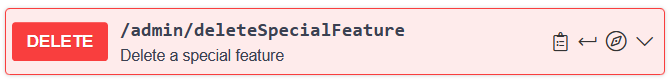
\includegraphics [width=1\textwidth] {images/andreas/praxis/deleteSF.png}
            \caption{Delete Route to Delete a Special Feature}
        \end{figure}

        \item \textbf{\texttt{DELETE /deleteAddress} - Delete an Address}
        \begin{itemize}
            \item This endpoint deletes an address from the system.
        \end{itemize} 
        \begin{figure} [H]
            \centering
            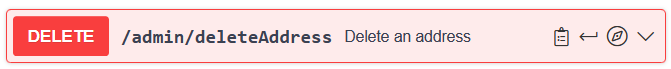
\includegraphics [width=1\textwidth] {images/andreas/praxis/deleteAddress.png}
            \caption{Delete Route to Delete an Address}
        \end{figure}
    \end{enumerate}
    \pagebreak